% Begin the document and set up the style of the document
\documentclass[a4paper,11pt]{article}

\usepackage{graphicx}
\usepackage{caption}

\usepackage{fullpage}

\usepackage{titlesec} % Used to customize the \section command
\titleformat{\section}{\bf}{}{0em}{}[\titlerule] % Text formatting of sections
\titlespacing*{\section}{0pt}{3pt}{3pt} % Spacing around sections

\usepackage{enumitem}

\newcommand{\indep}{\mathrel{\text{\scalebox{1.07}{$\perp\mkern-10mu\perp$}}}}
\newcommand{\ds}{\displaystyle}
\newcommand{\code}{\texttt}
\newcommand{\HRule}{\rule{\linewidth}{0.5mm}} % Defines a new command for the horizontal lines, change thickness here

\begin{document}

\begin{center}
	\LARGE \textbf{Lab 01 Report}
	\HRule\\
\end{center}

\pagenumbering{arabic}

\noindent \code{Lines in this font represent terminal commands and terminal output.}\\
Lines beginning with \code{\$} are the terminal commands that were run.\\
Lines in this font are the answers to the questions.

\section{EXERCISE 1}
\begin{enumerate}[leftmargin=*]
	\item 
		\code{\$ nslookup www.google.com\\
		Server:		129.94.242.2\\
		Address:	129.94.242.2\#53\\
		\newline
		Non-authoritative answer:\\
		Name:	www.google.com\\
		Address: 216.58.199.36\\}
		\newline
		The IP Address of Google is 216.58.199.36. Google uses multiple IP Addresses for load balancing, such that multiple servers have multiple IP Addresses to connect to based on traffic intensity and geographical location.
	\item 
		\code{\$ nslookup 127.0.0.1\\
		Server:		129.94.242.2\\
		Address:	129.94.242.2\#53\\
		\newline
		1.0.0.127.in-addr.arpa	name = localhost.\\}
		\newline
		The name of the IP Address 127.0.0.1 is localhost, it refers to the machine you are currently using, and is known as the loopback address. It allows you to point your software at your current computer without having to visit external routers over the network to find your current computer.
\end{enumerate}

\section{EXERCISE 2}
\code{\$ ping -c 3 www.cse.unsw.edu.au} -- Reachable by ping.\\
\newline
\code{\$ ping -c 3 www.getfittest.com.au}\\
\code{ping: unknown host www.getfittest.com.au}\\
Unreachable by ping. Unreachable by Web Browser as well, indicating that the host does not exist. The domain name does not have an IP Address associated with it.\\
\newline
\code{\$ ping -c 3 www.mit.edu.au} -- Reachable by ping.\\
\newline
\code{\$ ping -c 3 www.intel.com.au} -- Reachable by ping.\\
\newline
\code{\$ ping -c 3 www.tpg.com.au} -- Reachable by ping.\\
\newline
\code{\$ ping -c 3 www.hola.hp}\\
\code{ping: unknown host www.hola.hp}\\
Unreachable by ping. Unreachable by Web Browser as well, indicating that the host does not exist. The domain name does not have an IP Address associated with it.\\
\pagebreak\\
\code{\$ ping -c 3 www.amazon.com} -- Reachable by ping.\\
\newline
\code{\$ ping -c 3 www.tsinghua.edu.cn} -- Reachable by ping.\\
\newline
\code{\$ ping -c 3 www.kremlin.ru}\\
\code{PING www.kremlin.ru (95.173.136.70) 56(84) bytes of data.}\\
\code{--- www.kremlin.ru ping statistics ---}\\
\code{3 packets transmitted, 0 received, 100\% packet loss, time 2039ms}\\
All packets are dropped by the host, indicated by the 100\% packet loss. This usually indicates that the firewall of the host is set to drop all icmp ping requests. We can reasonably assume this is true, and thus the host is reachable, just not responding to the ping request. Using a Web Browser, we can reach the host.\\
\newline
\code{\$ ping -c 3 8.8.8.8} -- Reachable by ping.\\

\section{EXERCISE 3}
\begin{enumerate}[leftmargin=*]
	\item \code{\footnotesize \$ traceroute www.columbia.edu\\
			traceroute to www.columbia.edu (128.59.105.24), 30 hops max, 60 byte packets\\
		 1  cserouter1-server.cse.unsw.EDU.AU (129.94.242.251)  0.094 ms  0.084 ms  0.101 ms\\
		 2  129.94.39.17 (129.94.39.17)  0.991 ms  0.976 ms  1.016 ms\\
		 3  libudnex1-vl-3154.gw.unsw.edu.au (149.171.253.34)  1.495 ms\\
		 	ombudnex1-vl-3154.gw.unsw.edu.au (149.171.253.35)  1.588 ms  1.408 ms\\
		 4  libcr1-po-5.gw.unsw.edu.au (149.171.255.165)  1.185 ms ombcr1-po-5.gw.unsw.edu.au\\
		 (149.171.255.197)  1.300 ms  1.286 ms\\
		 5  unswbr1-te-2-13.gw.unsw.edu.au (149.171.255.105)  1.321 ms  1.340 ms\\
		 	unswbr1-te-1-9.gw.unsw.edu.au (149.171.255.101)  1.365 ms\\
		 6  138.44.5.0 (138.44.5.0)  1.525 ms  1.438 ms  1.436 ms\\
		 7  et-1-3-0.pe1.sxt.bkvl.nsw.aarnet.net.au (113.197.15.149)  2.453 ms  2.271 ms  2.251 ms\\
		 8  et-0-0-0.pe1.a.hnl.aarnet.net.au (113.197.15.99)  95.186 ms  95.289 ms  95.225 ms\\
		 9  et-2-1-0.bdr1.a.sea.aarnet.net.au (113.197.15.201)  146.762 ms  146.727 ms  146.695 ms\\
		10  abilene-1-lo-jmb-706.sttlwa.pacificwave.net (207.231.240.8)  146.980 ms  146.960 ms  146.690 ms\\
		11  et-4-0-0.4079.rtsw.miss2.net.internet2.edu (162.252.70.0)  157.787 ms  157.753 ms  157.799 ms\\
		12  et-4-0-0.4079.rtsw.minn.net.internet2.edu (162.252.70.58)  180.814 ms  180.673 ms  180.538 ms\\
		13  et-1-1-5.4079.rtsw.eqch.net.internet2.edu (162.252.70.106)  188.527 ms  189.856 ms  189.722 ms\\
		14  162.252.70.163 (162.252.70.163)  188.541 ms  188.907 ms  190.028 ms\\
		15  ae-1.4079.rtsw.clev.net.internet2.edu (162.252.70.130)  197.265 ms  197.291 ms  197.272 ms\\
		16  buf-9208-I2-CLEV.nysernet.net (199.109.11.33)  201.413 ms  201.520 ms  201.438 ms\\
		17  syr-9208-buf-9208.nysernet.net (199.109.7.193)  204.777 ms  204.869 ms  204.894 ms\\
		18  nyc-9208-syr-9208.nysernet.net (199.109.7.162)  210.574 ms  210.862 ms  210.536 ms\\
		19  columbia.nyc-9208.nysernet.net (199.109.4.14)  210.400 ms  210.535 ms  210.529 ms\\
		20  cc-core-1-x-nyser32-gw-1.net.columbia.edu (128.59.255.5)  210.635 ms  210.853 ms  210.796 ms\\
		21  cc-conc-1-x-cc-core-1.net.columbia.edu (128.59.255.210)  210.775 ms  210.808 ms  210.737 ms\\
	22  neurotheory.columbia.edu (128.59.105.24)  210.617 ms  210.844 ms  210.733 ms\\}

	There are 22 routers between the CSE computer and the destination host. 5 routers are a part of the UNSW network, routers 1-5. Considering the time taken for pings to reach the router and return, we can identify the point that the packets cross the Pacific. The time taken to ping router 8 (95 ms) compared with the time taken to ping router 7 (2.3 ms) indicates a large distance crossed beteen those two routers. Furthermore, the time taken to ping router 9 (147 ms) compared to the time taken to ping router 8 (95 ms) is still a significant change, although not as large a difference as between routers 7 and 8. This large difference in times indicates that the packets cross the Pacific Ocean between routers 7 and 9, with router 8 being an intermediary hop about two-thirds the way across the Pacific. Looking at a map, this lines up with router 8 being on Haiwaii, which is situated about two-thirds of the way from Australia to mainland US.
	\item 
		\begin{enumerate}
			\item \code{\scriptsize \$ traceroute www.ucla.edu\\
			traceroute to www.ucla.edu (164.67.228.152), 30 hops max, 60 byte packets\\
			 1  cserouter1-server.cse.unsw.EDU.AU (129.94.242.251)  0.135 ms  0.107 ms  0.122 ms\\
			 2  129.94.39.17 (129.94.39.17)  1.075 ms  1.051 ms  1.022 ms\\
			 3  libudnex1-vl-3154.gw.unsw.edu.au (149.171.253.34)  1.858 ms  1.842 ms\\
			 ombudnex1-vl-3154.gw.unsw.edu.au (149.171.253.35)  1.625 ms\\
			 4  libcr1-po-5.gw.unsw.edu.au (149.171.255.165)  1.216 ms ombcr1-po-6.gw.unsw.edu.au\\
			 (149.171.255.169)  1.294 ms ombcr1-po-5.gw.unsw.edu.au (149.171.255.197)  1.275 ms\\
			 5  unswbr1-te-1-9.gw.unsw.edu.au (149.171.255.101)  1.367 ms  1.507 ms  1.490 ms\\
			 6  138.44.5.0 (138.44.5.0)  1.896 ms  1.664 ms  1.640 ms\\
			 7  et-1-3-0.pe1.sxt.bkvl.nsw.aarnet.net.au (113.197.15.149)  2.605 ms  2.367 ms  2.378 ms\\
			 8  et-0-0-0.pe1.a.hnl.aarnet.net.au (113.197.15.99)  95.319 ms  95.343 ms  95.338 ms\\
			 9  et-2-1-0.bdr1.a.sea.aarnet.net.au (113.197.15.201)  146.855 ms  146.784 ms  146.705 ms\\
			10  cenichpr-1-is-jmb-778.snvaca.pacificwave.net (207.231.245.129)  163.168 ms  163.259 ms\\
			163.166 ms\\
			11  hpr-lax-hpr3--svl-hpr3-100ge.cenic.net (137.164.25.73)  171.067 ms  171.110 ms  171.108 ms\\
			12  * * *\\
			13  bd11f1.anderson--cr00f2.csb1.ucla.net (169.232.4.4)  173.503 ms\\
			bd11f1.anderson--cr001.anderson.ucla.net (169.232.4.6)  171.511 ms\\
			bd11f1.anderson--cr00f2.csb1.ucla.net (169.232.4.4)  171.549 ms\\
			14  cr00f2.csb1--dr00f2.csb1.ucla.net (169.232.4.53)  171.438 ms  171.522 ms\\
			cr00f1.anderson--dr00f2.csb1.ucla.net (169.232.4.55)  171.535 ms\\}
		\item \code{\scriptsize \$ traceroute www.u-tokyo.ac.jp\\
			traceroute to www.u-tokyo.ac.jp (210.152.243.234), 30 hops max, 60 byte packets\\
			 1  cserouter1-server.cse.unsw.EDU.AU (129.94.242.251)  0.108 ms  0.089 ms  0.112 ms\\
			 2  129.94.39.17 (129.94.39.17)  1.101 ms  1.066 ms  1.052 ms\\
			 3  ombudnex1-vl-3154.gw.unsw.edu.au (149.171.253.35)  1.544 ms\\
			 libudnex1-vl-3154.gw.unsw.edu.au (149.171.253.34)  1.655 ms  1.634 ms\\
			 4  ombcr1-po-6.gw.unsw.edu.au (149.171.255.169)  1.244 ms libcr1-po-5.gw.unsw.edu.au\\
			 (149.171.255.165)  1.239 ms libcr1-po-6.gw.unsw.edu.au (149.171.255.201)  1.254 ms\\
			 5  unswbr1-te-2-13.gw.unsw.edu.au (149.171.255.105)  1.269 ms  1.404 ms  1.377 ms\\
			 6  138.44.5.0 (138.44.5.0)  1.527 ms  1.467 ms  1.625 ms\\
			 7  et-0-3-0.pe1.bkvl.nsw.aarnet.net.au (113.197.15.147)  1.959 ms  1.904 ms  1.919 ms\\
			 8  ge-4\_0\_0.bb1.a.pao.aarnet.net.au (202.158.194.177)  156.213 ms  156.130 ms  156.315 ms\\
			 9  paloalto0.iij.net (198.32.176.24)  158.160 ms  158.202 ms  158.020 ms\\
			10  osk004bb01.IIJ.Net (58.138.88.189)  271.335 ms  271.205 ms osk004bb00.IIJ.Net (58.138.88.185)\\ 
			288.958 ms\\
			11  osk004ix51.IIJ.Net (58.138.106.130)  279.662 ms osk004ix51.IIJ.Net (58.138.106.126)\\
			288.581 ms osk004ix51.IIJ.Net (58.138.106.130)  279.720 ms\\
			12  210.130.135.130 (210.130.135.130)  288.548 ms  288.458 ms  288.451 ms\\
			13  124.83.228.58 (124.83.228.58)  292.545 ms  345.384 ms  345.344 ms\\
			14  124.83.252.178 (124.83.252.178)  277.117 ms  277.035 ms  277.010 ms\\
			15  158.205.134.26 (158.205.134.26)  285.702 ms  285.791 ms  285.694 ms\\}
		\item \code{\scriptsize \$ traceroute www.lancaster.ac.uk\\
			traceroute to www.lancaster.ac.uk (148.88.65.80), 30 hops max, 60 byte packets\\
			 1  cserouter1-server.cse.unsw.EDU.AU (129.94.242.251)  0.146 ms  0.122 ms  0.102 ms\\
			 2  129.94.39.17 (129.94.39.17)  1.101 ms  1.066 ms  1.056 ms\\
			 3  libudnex1-vl-3154.gw.unsw.edu.au (149.171.253.34)  1.747 ms  1.693 ms\\
			 ombudnex1-vl-3154.gw.unsw.edu.au (149.171.253.35)  1.352 ms\\
			 4  ombcr1-po-6.gw.unsw.edu.au (149.171.255.169)  34.273 ms\\
			 ombcr1-po-5.gw.unsw.edu.au (149.171.255.197)  34.232 ms  34.279 ms\\
			 5  unswbr1-te-2-13.gw.unsw.edu.au (149.171.255.105)  1.380 ms\\
			 unswbr1-te-1-9.gw.unsw.edu.au (149.171.255.101)  1.262 ms  1.294 ms\\
			 6  138.44.5.0 (138.44.5.0)  1.442 ms  1.415 ms  1.515 ms\\
			 7  et-1-3-0.pe1.sxt.bkvl.nsw.aarnet.net.au (113.197.15.149)  2.521 ms  2.247 ms  2.187 ms\\
			 8  et-0-0-0.pe1.a.hnl.aarnet.net.au (113.197.15.99)  95.228 ms  95.276 ms  95.312 ms\\
			 9  et-2-1-0.bdr1.a.sea.aarnet.net.au (113.197.15.201)  146.683 ms  146.667 ms  146.610 ms\\
			10  abilene-1-lo-jmb-706.sttlwa.pacificwave.net (207.231.240.8)  146.845 ms  146.756 ms  146.713 ms\\
			11  et-4-0-0.4079.rtsw.miss2.net.internet2.edu (162.252.70.0)  158.187 ms  158.458 ms  158.147 ms\\
			12  et-4-0-0.4079.rtsw.minn.net.internet2.edu (162.252.70.58)  180.600 ms  180.848 ms  180.620 ms\\
			13  et-1-1-5.4079.rtsw.eqch.net.internet2.edu (162.252.70.106)  188.590 ms  188.796 ms  188.571 ms\\
			14  162.252.70.163 (162.252.70.163)  189.182 ms  189.217 ms  197.162 ms\\
			15  ae-1.4079.rtsw.clev.net.internet2.edu (162.252.70.130)  198.321 ms  198.084 ms  198.200 ms\\
			16  et-2-0-0.4079.rtsw.ashb.net.internet2.edu (162.252.70.54)  205.072 ms  206.060 ms  205.944 ms\\
			17  ae-2.4079.rtsw.wash.net.internet2.edu (162.252.70.136)  206.244 ms  205.340 ms  205.310 ms\\
			18  internet2-gw.mx1.lon.uk.geant.net (62.40.124.44)  280.398 ms  280.364 ms  280.379 ms\\
			19  janet-gw.mx1.lon.uk.geant.net (62.40.124.198)  280.625 ms  280.737 ms  283.460 ms\\
			20  ae29.londpg-sbr2.ja.net (146.97.33.2)  300.343 ms  299.030 ms  298.981 ms\\
			21  ae31.erdiss-sbr2.ja.net (146.97.33.22)  284.975 ms  284.773 ms  284.754 ms\\
			22  ae29.manckh-sbr2.ja.net (146.97.33.42)  286.605 ms  286.655 ms  286.659 ms\\
			23  ae24.lanclu-rbr1.ja.net (146.97.38.58)  288.977 ms  288.832 ms  288.898 ms\\
			24  lancaster-university.ja.net (194.81.46.2)  305.054 ms  304.661 ms  304.051 ms\\
			25  * * *\\
			26  ismx-issrx.rtr.lancs.ac.uk (148.88.255.17)  290.729 ms  290.703 ms  290.655 ms\\
			27  dc.iss.srv.rtrcloud.lancs.ac.uk (148.88.253.3)  305.025 ms  302.714 ms  302.355 ms\\
			28  www.lancs.ac.uk (148.88.65.80)  290.579 ms !X  290.952 ms !X  290.519 ms !X\\}
		\end{enumerate}

		All three paths to the destination hosts diverge at router 6, with IP Address 138.44.5.0. Using the \code{whois} command, router 6 is managed by Australian Academic and Research Network. This router is probably linked to ingoing and outgoing connections from/to Australian university and academic networks. This router is used by UNSW, but not necessarily owned by UNSW, or a part of the UNSW Network.\\
		\break
		The distance from Sydney to California is roughly 12000km, and has 14 routers in the path. The distance from Sydney to Tokyo is roughly 7000km, and has 15 routers in the path. The distance from Sydney to Lancaster is roughly 17000km, and has 28 routers in the path. This does not show any simple proporionality relationship between the number of hop routers and the geographical distance.\\
		\break
		There are many hops within the UNSW network, however to cross the Pacific Ocean, only one intermediary hop was required. This also demonstrates that there is NOT a proporionality relationship between the number of routers and the physical distance traversed.\\
	\item
		\begin{enumerate}
			\item From www.speedtest.sg/tr.php to my machine.\\
				\code{\scriptsize traceroute to 129.94.242.53 (129.94.242.53), 30 hops max, 60 byte packets\\
				 1  ge2-8.r01.sin01.ne.com.sg (202.150.221.169)  0.156 ms  0.178 ms  0.184 ms\\
				 2  10.11.33.30 (10.11.33.30)  0.252 ms  0.262 ms  0.272 ms\\
				 3  10.11.33.74 (10.11.33.74)  0.722 ms  0.730 ms  0.735 ms\\
				 4  aarnet.sgix.sg (103.16.102.67)  225.643 ms  225.702 ms  225.682 ms\\
				 5  xe-3-0-3.pe1.brwy.nsw.aarnet.net.au (113.197.15.206)  232.785 ms  232.829 ms  232.803 ms\\
				 6  138.44.5.1 (138.44.5.1)  225.853 ms  225.959 ms  225.852 ms\\
				 7  libcr1-te-1-5.gw.unsw.edu.au (149.171.255.102)  225.944 ms  225.955 ms  226.067 ms\\
				 8  ombudnex1-po-1.gw.unsw.edu.au (149.171.255.202)  236.584 ms  236.601 ms libudnex1-po-1.gw.unsw.edu.au (149.171.255.166)  224.150 ms\\
				 9  ufw1-ae-1-3154.gw.unsw.edu.au (149.171.253.36)  236.534 ms  236.470 ms  236.488 ms\\
				10  129.94.39.23 (129.94.39.23)  224.734 ms  224.759 ms  224.886 ms\\}
				\break
				From my machine to www.speedtest.sg.\\
				\code{\scriptsize \$ traceroute www.speedtest.sg\\
				traceroute to www.speedtest.com.sg (202.150.221.170), 30 hops max, 60 byte packets\\
				 1  cserouter1-server.cse.unsw.EDU.AU (129.94.242.251)  0.131 ms  0.106 ms  0.091 ms\\
				 2  129.94.39.17 (129.94.39.17)  1.115 ms  1.086 ms  1.074 ms\\
				 3  libudnex1-vl-3154.gw.unsw.edu.au (149.171.253.34)  1.619 ms ombudnex1-vl-3154.gw.unsw.edu.au\\
				 (149.171.253.35)  1.944 ms  2.749 ms\\
				 4  libcr1-po-6.gw.unsw.edu.au (149.171.255.201)  1.275 ms ombcr1-po-6.gw.unsw.edu.au (149.171.255.169)  1.256 ms  1.264 ms\\
				 5  unswbr1-te-2-13.gw.unsw.edu.au (149.171.255.105)  1.348 ms  1.384 ms  1.306 ms\\
				 6  138.44.5.0 (138.44.5.0)  1.456 ms  1.401 ms  1.418 ms\\
				 7  et-0-3-0.pe1.alxd.nsw.aarnet.net.au (113.197.15.153)  2.055 ms  1.871 ms  2.011 ms\\
				 8  xe-0-2-1-204.pe1.wnpa.alxd.aarnet.net.au (113.197.15.183)  24.354 ms  24.344 ms\\
				 xe-0-0-3.pe1.wnpa.akl.aarnet.net.au (113.197.15.67)  24.322 ms\\
				 9  et-0-1-0.200.pe1.tkpa.akl.aarnet.net.au (113.197.15.69)  24.684 ms  24.728 ms  24.708 ms\\
				10  xe-0-2-6.bdr1.a.lax.aarnet.net.au (202.158.194.173)  148.076 ms  148.187 ms  148.036 ms\\
				11  singtel.as7473.any2ix.coresite.com (206.72.210.63)  148.247 ms  148.160 ms  148.160 ms\\
				12  203.208.151.181 (203.208.151.181)  317.311 ms 203.208.171.9 (203.208.171.9)  320.224 ms 203.208.172.173 (203.208.172.173)  148.316 ms\\
				13  203.208.177.110 (203.208.177.110)  236.757 ms  224.933 ms 203.208.151.233 (203.208.151.233)\\
				308.023 ms\\
			14  202-150-221-170.rev.ne.com.sg (202.150.221.170)  237.043 ms 203.208.182.45 (203.208.182.45)  334.005 ms 202-150-221-170.rev.ne.com.sg (202.150.221.170)  224.793 ms\\}

		\pagebreak

		\item From www.telstra.net/cgi-bin/trace to my machine.\\
			\code{\scriptsize 1  gigabitethernet3-3.exi2.melbourne.telstra.net (203.50.77.53)  0.247 ms  0.223 ms  0.242 ms\\
 2  bundle-ether3-100.win-core10.melbourne.telstra.net (203.50.80.129)  1.118 ms  1.862 ms  1.868 ms\\
 3  bundle-ether12.ken-core10.sydney.telstra.net (203.50.11.122)  12.738 ms  12.356 ms  12.987 ms\\
 4  bundle-ether1.ken-edge901.sydney.telstra.net (203.50.11.95)  12.112 ms  13.229 ms  11.862 ms\\
 5  aarnet6.lnk.telstra.net (139.130.0.78)  11.609 ms  11.607 ms  11.609 ms\\
 6  ge-6-0-0.bb1.a.syd.aarnet.net.au (202.158.202.17)  11.862 ms  11.729 ms  11.737 ms\\
 7  ae9.pe2.brwy.nsw.aarnet.net.au (113.197.15.56)  11.985 ms  12.103 ms  11.986 ms\\
 8  et-3-1-0.pe1.brwy.nsw.aarnet.net.au (113.197.15.146)  12.111 ms  12.107 ms  12.111 ms\\
 9  138.44.5.1 (138.44.5.1)  12.360 ms  12.356 ms  12.362 ms\\
10  libcr1-te-1-5.gw.unsw.edu.au (149.171.255.102)  12.360 ms  12.357 ms  12.361 ms\\
11  libudnex1-po-1.gw.unsw.edu.au (149.171.255.166)  12.615 ms  12.608 ms  12.608 ms\\
12  ufw1-ae-1-3154.gw.unsw.edu.au (149.171.253.36)  13.110 ms  13.106 ms  12.986 ms\\
13  129.94.39.23 (129.94.39.23)  13.236 ms  13.232 ms  13.237 ms\\}
			\break
			From my machine to www.telstra.net/cgi-bin/trace.\\
			\code{\scriptsize \$ traceroute www.telstra.net\\
			traceroute to www.telstra.net (203.50.5.178), 30 hops max, 60 byte packets\\
			 1  cserouter1-server.cse.unsw.EDU.AU (129.94.242.251)  0.127 ms  0.115 ms  0.097 ms\\
			 2  129.94.39.17 (129.94.39.17)  1.087 ms  1.050 ms  1.028 ms\\
			 3  libudnex1-vl-3154.gw.unsw.edu.au (149.171.253.34)  1.824 ms ombudnex1-vl-3154.gw.unsw.edu.au\\
			 (149.171.253.35)  1.577 ms libudnex1-vl-3154.gw.unsw.edu.au (149.171.253.34)  1.630 ms\\
			 4  libcr1-po-5.gw.unsw.edu.au (149.171.255.165)  1.364 ms libcr1-po-6.gw.unsw.edu.au\\
			 (149.171.255.201)  1.417 ms ombcr1-po-5.gw.unsw.edu.au (149.171.255.197)  1.219 ms\\
			 5  unswbr1-te-2-13.gw.unsw.edu.au (149.171.255.105)  1.324 ms unswbr1-te-1-9.gw.unsw.edu.au\\
			 (149.171.255.101)  1.312 ms unswbr1-te-2-13.gw.unsw.edu.au (149.171.255.105)  1.363 ms\\
			 6  138.44.5.0 (138.44.5.0)  1.394 ms  1.497 ms  1.488 ms\\
			 7  et-0-3-0.pe1.alxd.nsw.aarnet.net.au (113.197.15.153)  14.045 ms  13.378 ms  13.360 ms\\
			 8  ae9.bb1.b.syd.aarnet.net.au (113.197.15.65)  1.997 ms  1.916 ms  1.990 ms\\
			 9  gigabitethernet1-1.pe1.b.syd.aarnet.net.au (202.158.202.18)  1.974 ms  2.017 ms  1.948 ms\\
			10  gigabitethernet3-11.ken37.sydney.telstra.net (139.130.0.77)  4.281 ms  2.484 ms  2.585 ms\\
			11  bundle-ether2.chw-edge901.sydney.telstra.net (203.50.11.103)  2.694 ms\\
			bundle-ether13.ken-core10.sydney.telstra.net (203.50.11.94)  4.275 ms  4.235 ms\\
			12  bundle-ether10.win-core10.melbourne.telstra.net (203.50.11.123)  14.828 ms  14.791 ms\\
			bundle-ether13.chw-core10.sydney.telstra.net (203.50.11.98)  3.355 ms\\
			13  203.50.6.40 (203.50.6.40)  15.601 ms bundle-ether8.exi-core10.melbourne.telstra.net\\
			(203.50.11.125)  16.358 ms 203.50.6.40 (203.50.6.40)  15.584 ms\\
			14  bundle-ether2.exi-ncprouter101.melbourne.telstra.net (203.50.11.209)  15.560 ms  15.043 ms\\
			15.384 ms\\
			15  www.telstra.net (203.50.5.178)  14.374 ms  14.663 ms  15.047 ms\\}
			\break
			The IP Address of www.speedtest.sg is 202.150.221.170, and the IP Address of www.telstra.net is 203.50.5.178. The reverse and forward paths share a good amount of routers, but do have a few variations. For the routers that are shared between the two paths, they do not have the same IP Addresses, although in most cases they differ by 1 number in the very last section of the IP Address, ie, 149.171.255.165 for the forward direction and 149.171.255.166 for the reverse direction. This is due to multiple servers at the hop, some that manage outbound traffic, and some that manage inbound traffic, to share, and distribute the load.\\
		\end{enumerate}
\end{enumerate}

\section{EXERCISE 4}
		\begin{figure}[!htb]
		    \centering
			\begin{minipage}{\textwidth}
		        \centering
		        \captionof{figure}{Delay of www.nus.edu.sg vs Packet Number}
		        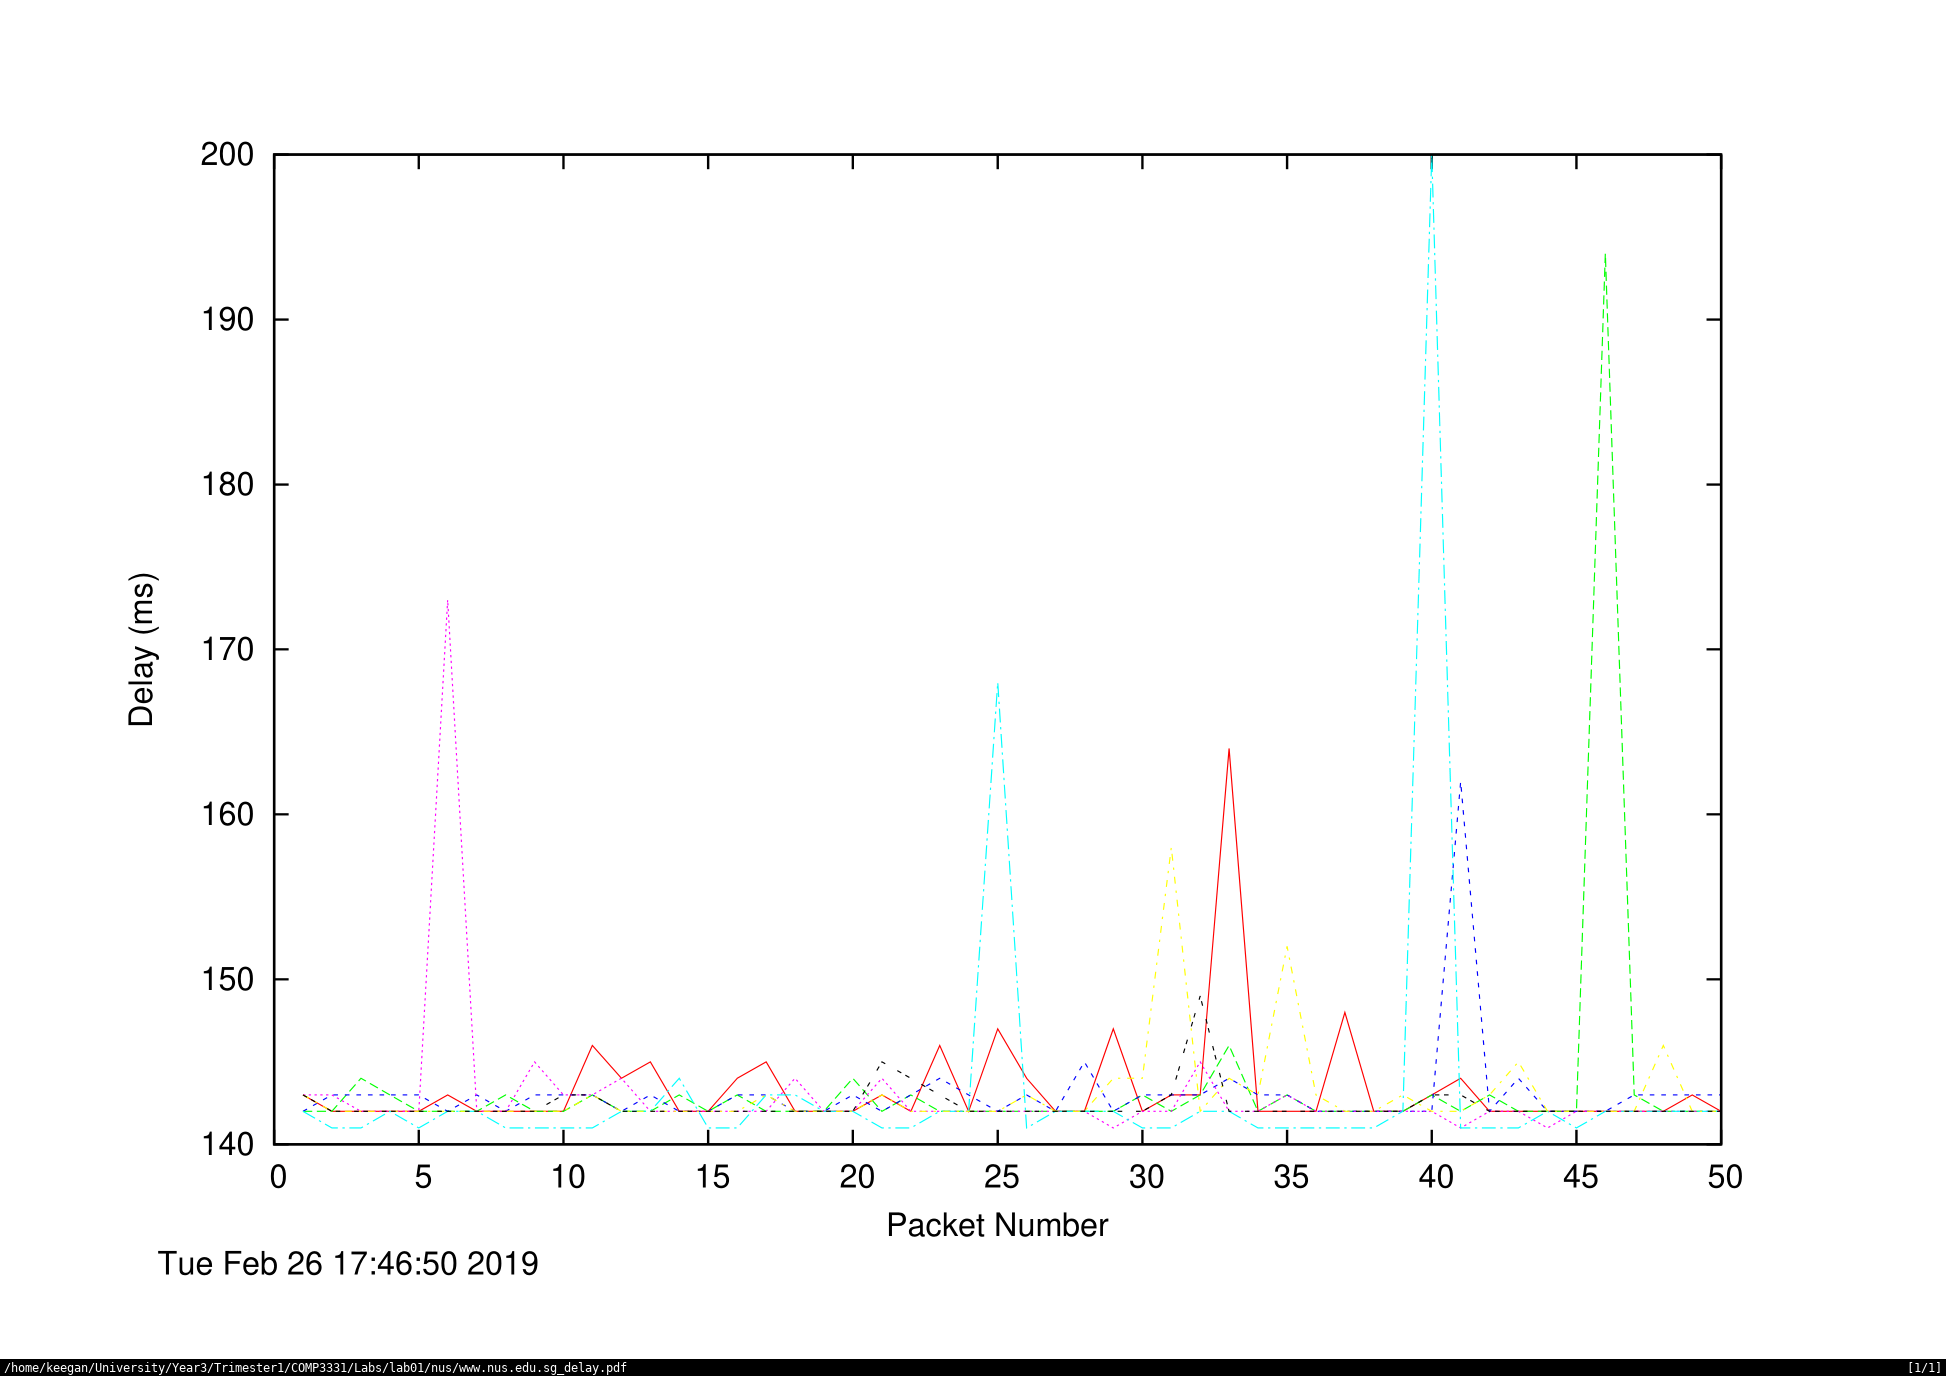
\includegraphics[width=\linewidth, height=0.4\textheight]{nusdelay.png}
		    \end{minipage}%
		\end{figure}

		\begin{figure}[!htb]
			\centering
			\begin{minipage}{\textwidth}
		        \centering
		        \captionof{figure}{Scatter of www.nus.edu.sg vs Packet Size}
		        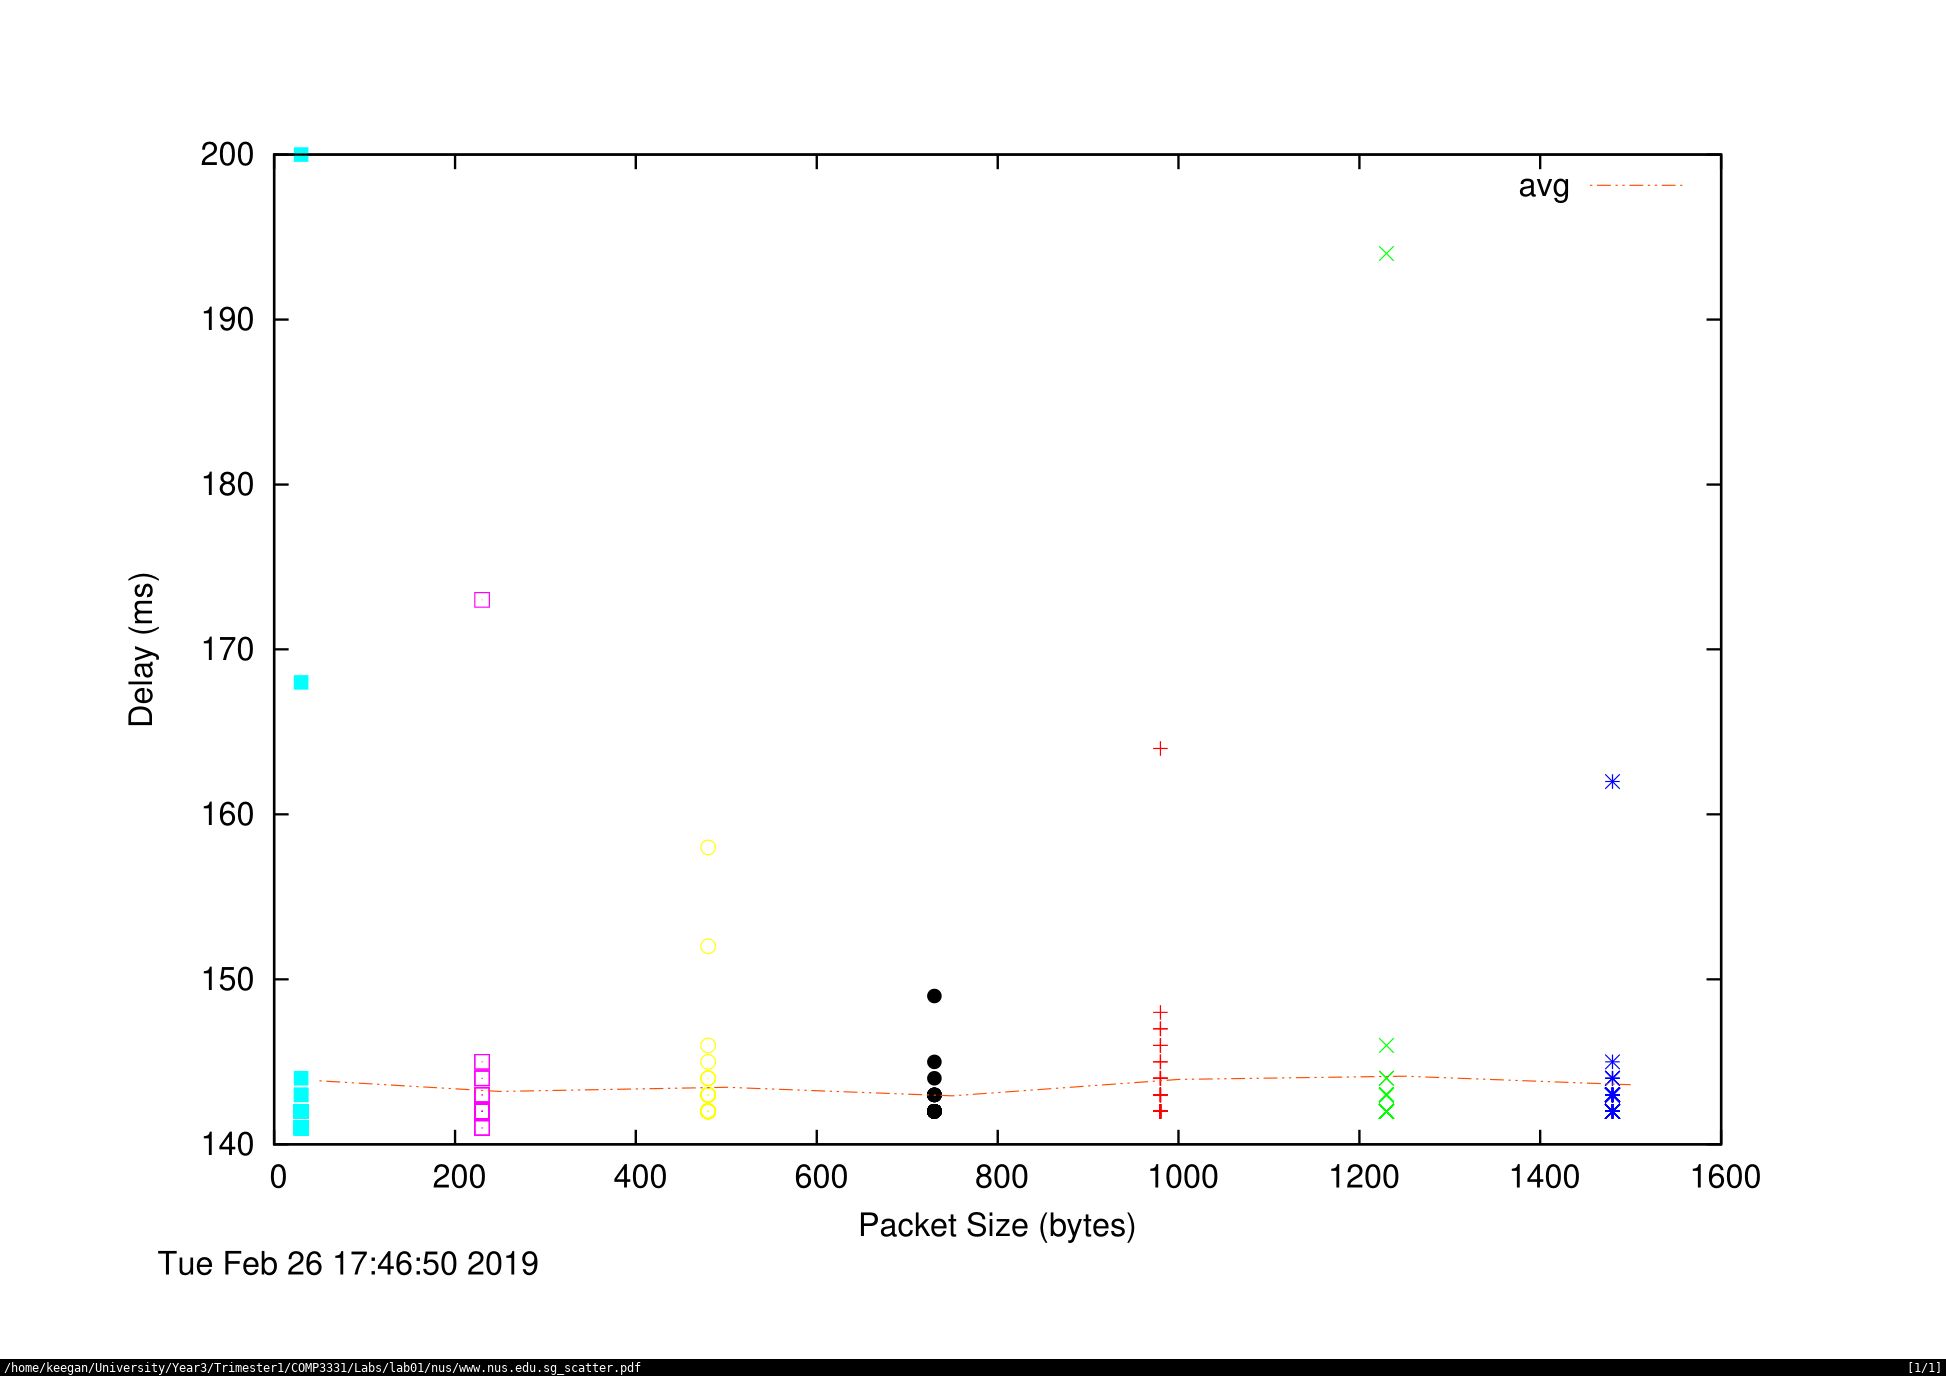
\includegraphics[width=\linewidth, height=0.4\textheight]{nusscatter.png}
		    \end{minipage}
		\end{figure}

		\begin{figure}[!htb]
		    \centering
		    \begin{minipage}{\textwidth}
		        \centering
		        \captionof{figure}{Delay of www.tu-berlin.de vs Packet Number}
		        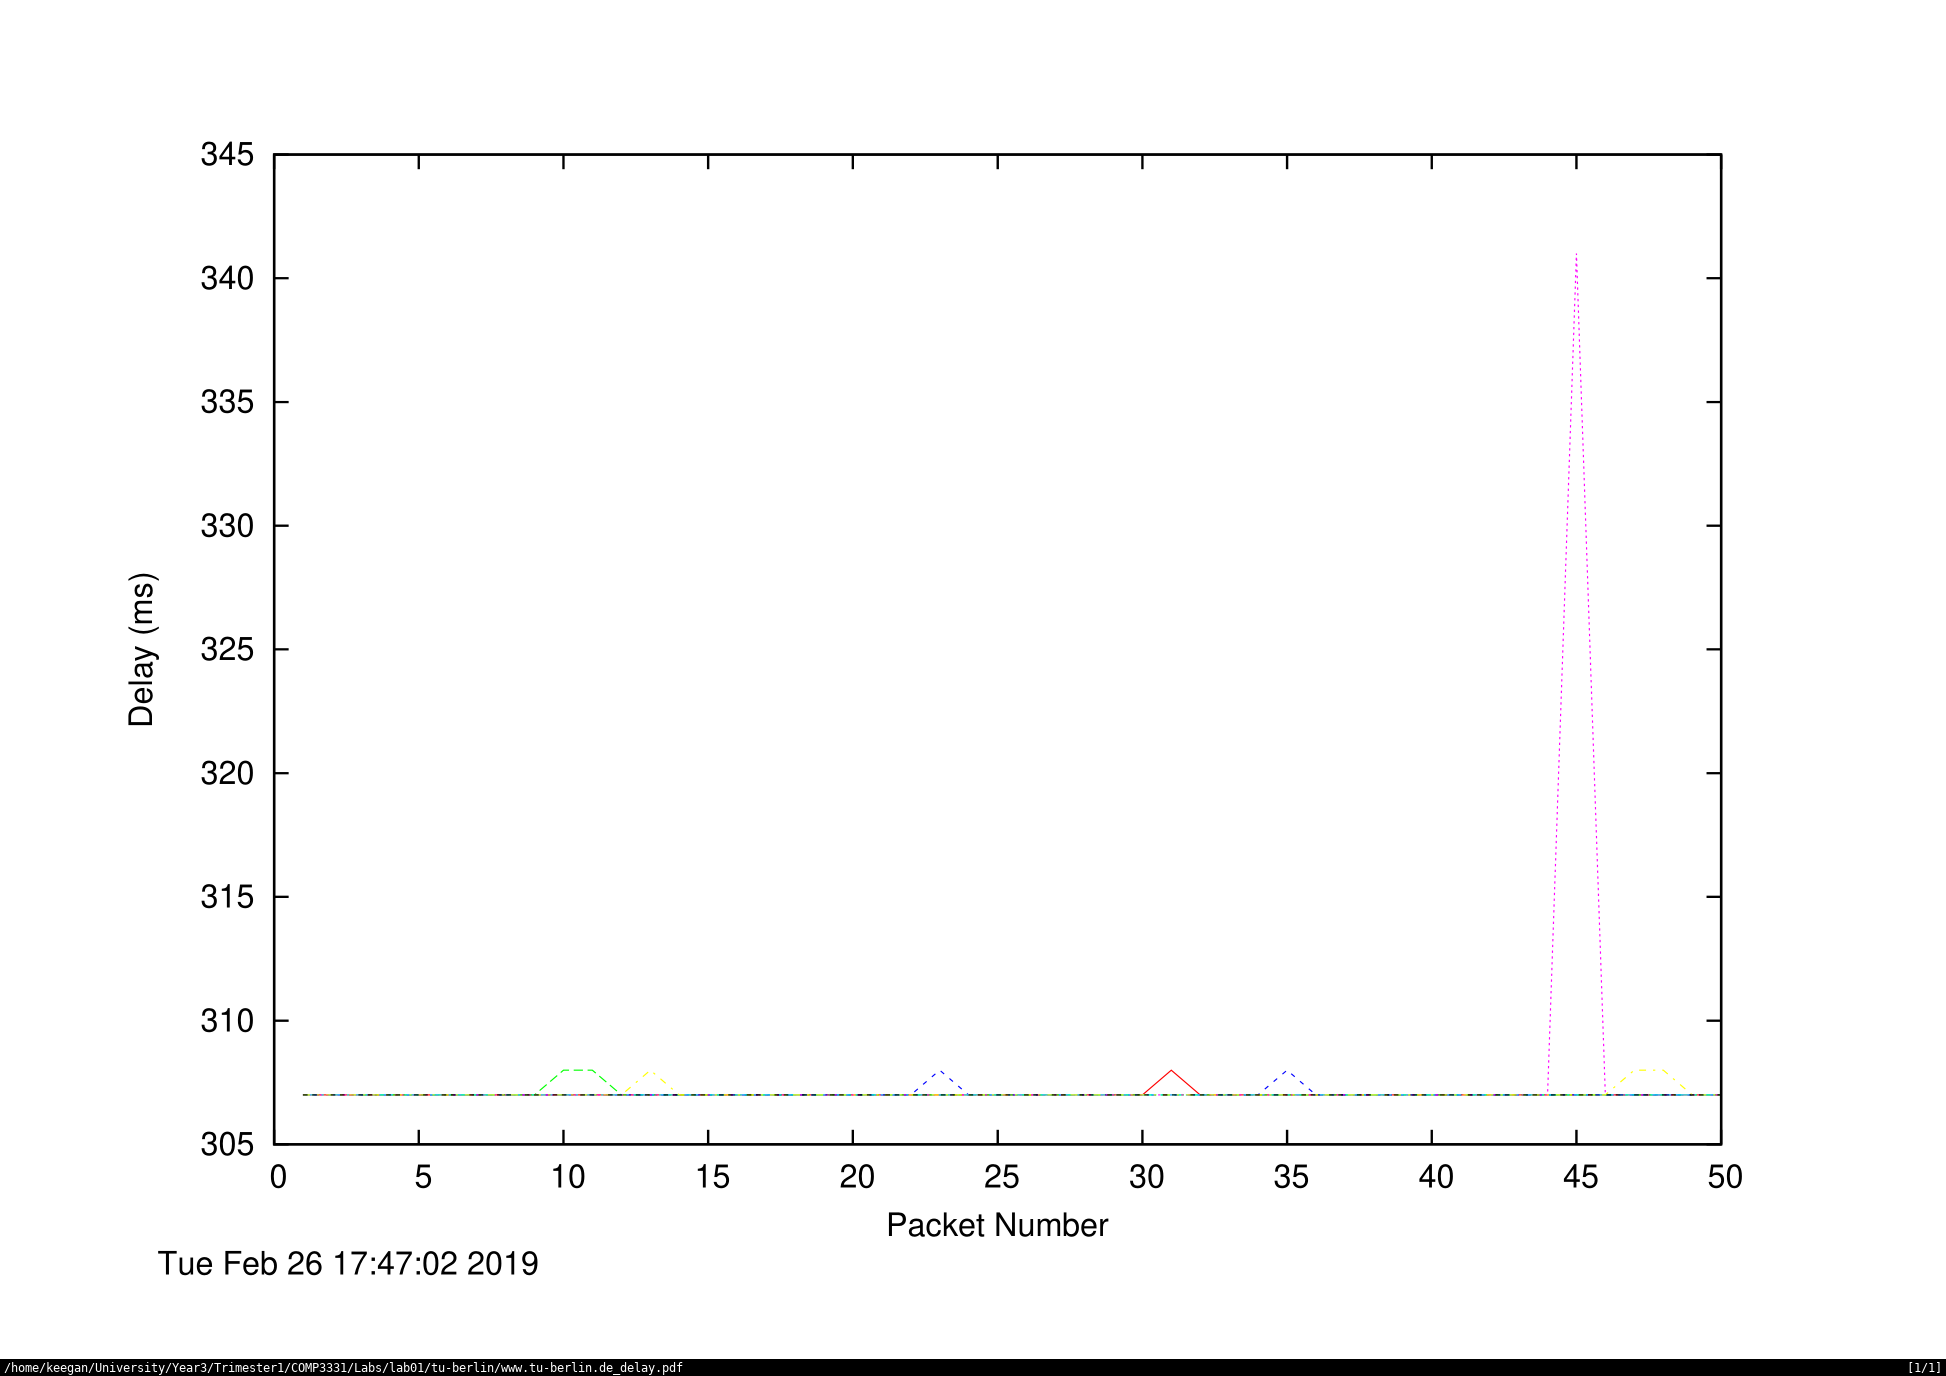
\includegraphics[width=\linewidth, height=0.43\textheight]{tuberlindelay.png}
		    \end{minipage}%
		\end{figure}

		\begin{figure}[!htb]
			\centering
		    \begin{minipage}{\textwidth}
		        \centering
		        \captionof{figure}{Scatter of www.tu-berlin.de vs Packet Size}
		        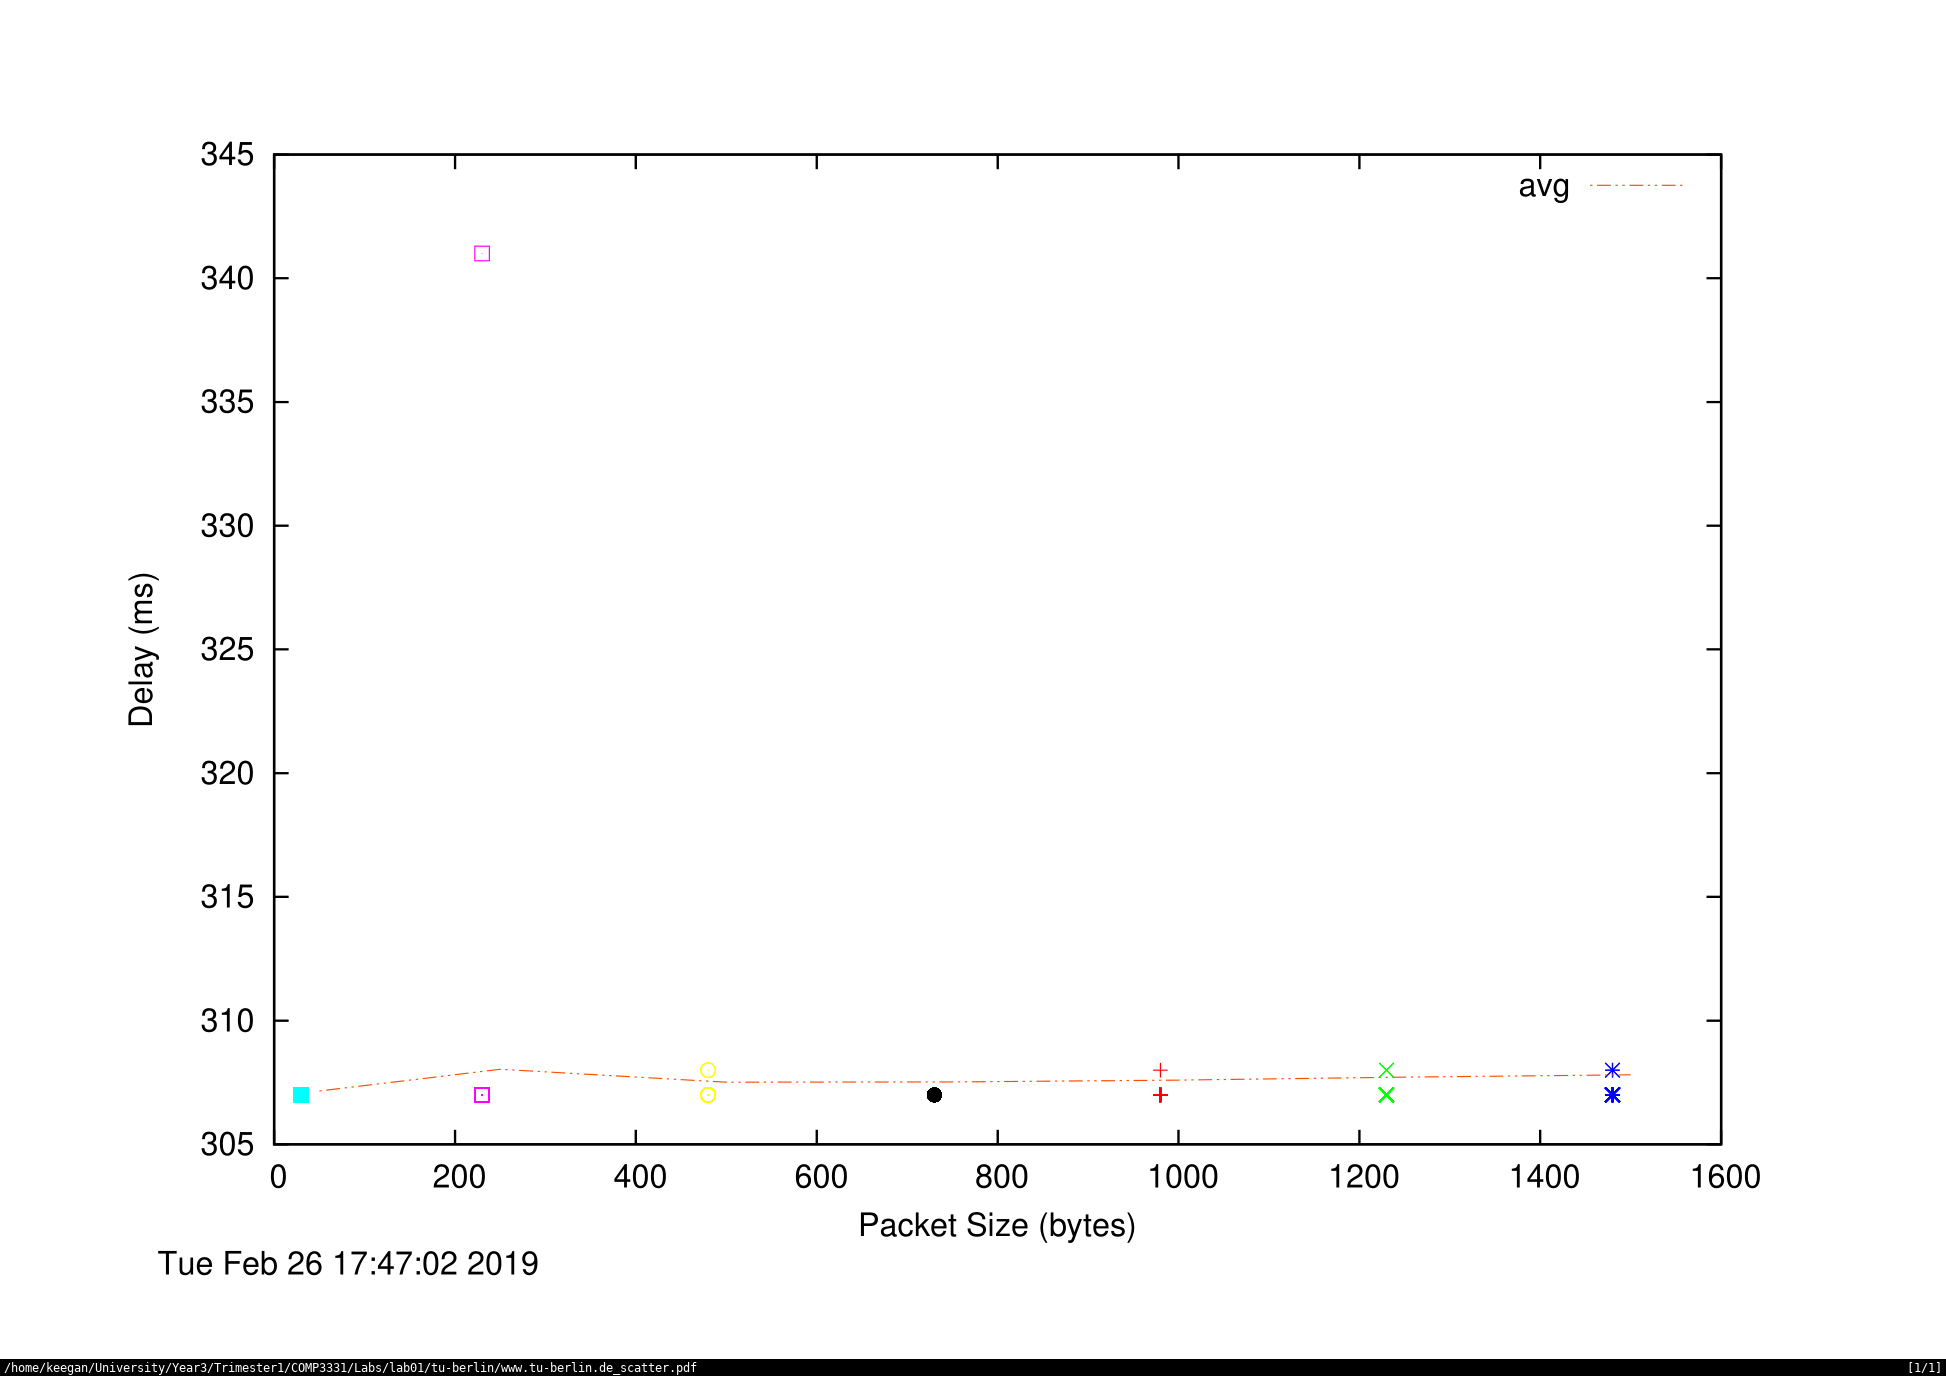
\includegraphics[width=\linewidth, height=0.43\textheight]{tuberlinscatter.png}
		    \end{minipage}
		\end{figure}

		\begin{figure}[!htb]
			\centering
		    \begin{minipage}{\textwidth}
		        \centering
		        \captionof{figure}{Delay of www.uq.edu.au vs Packet Number}
		        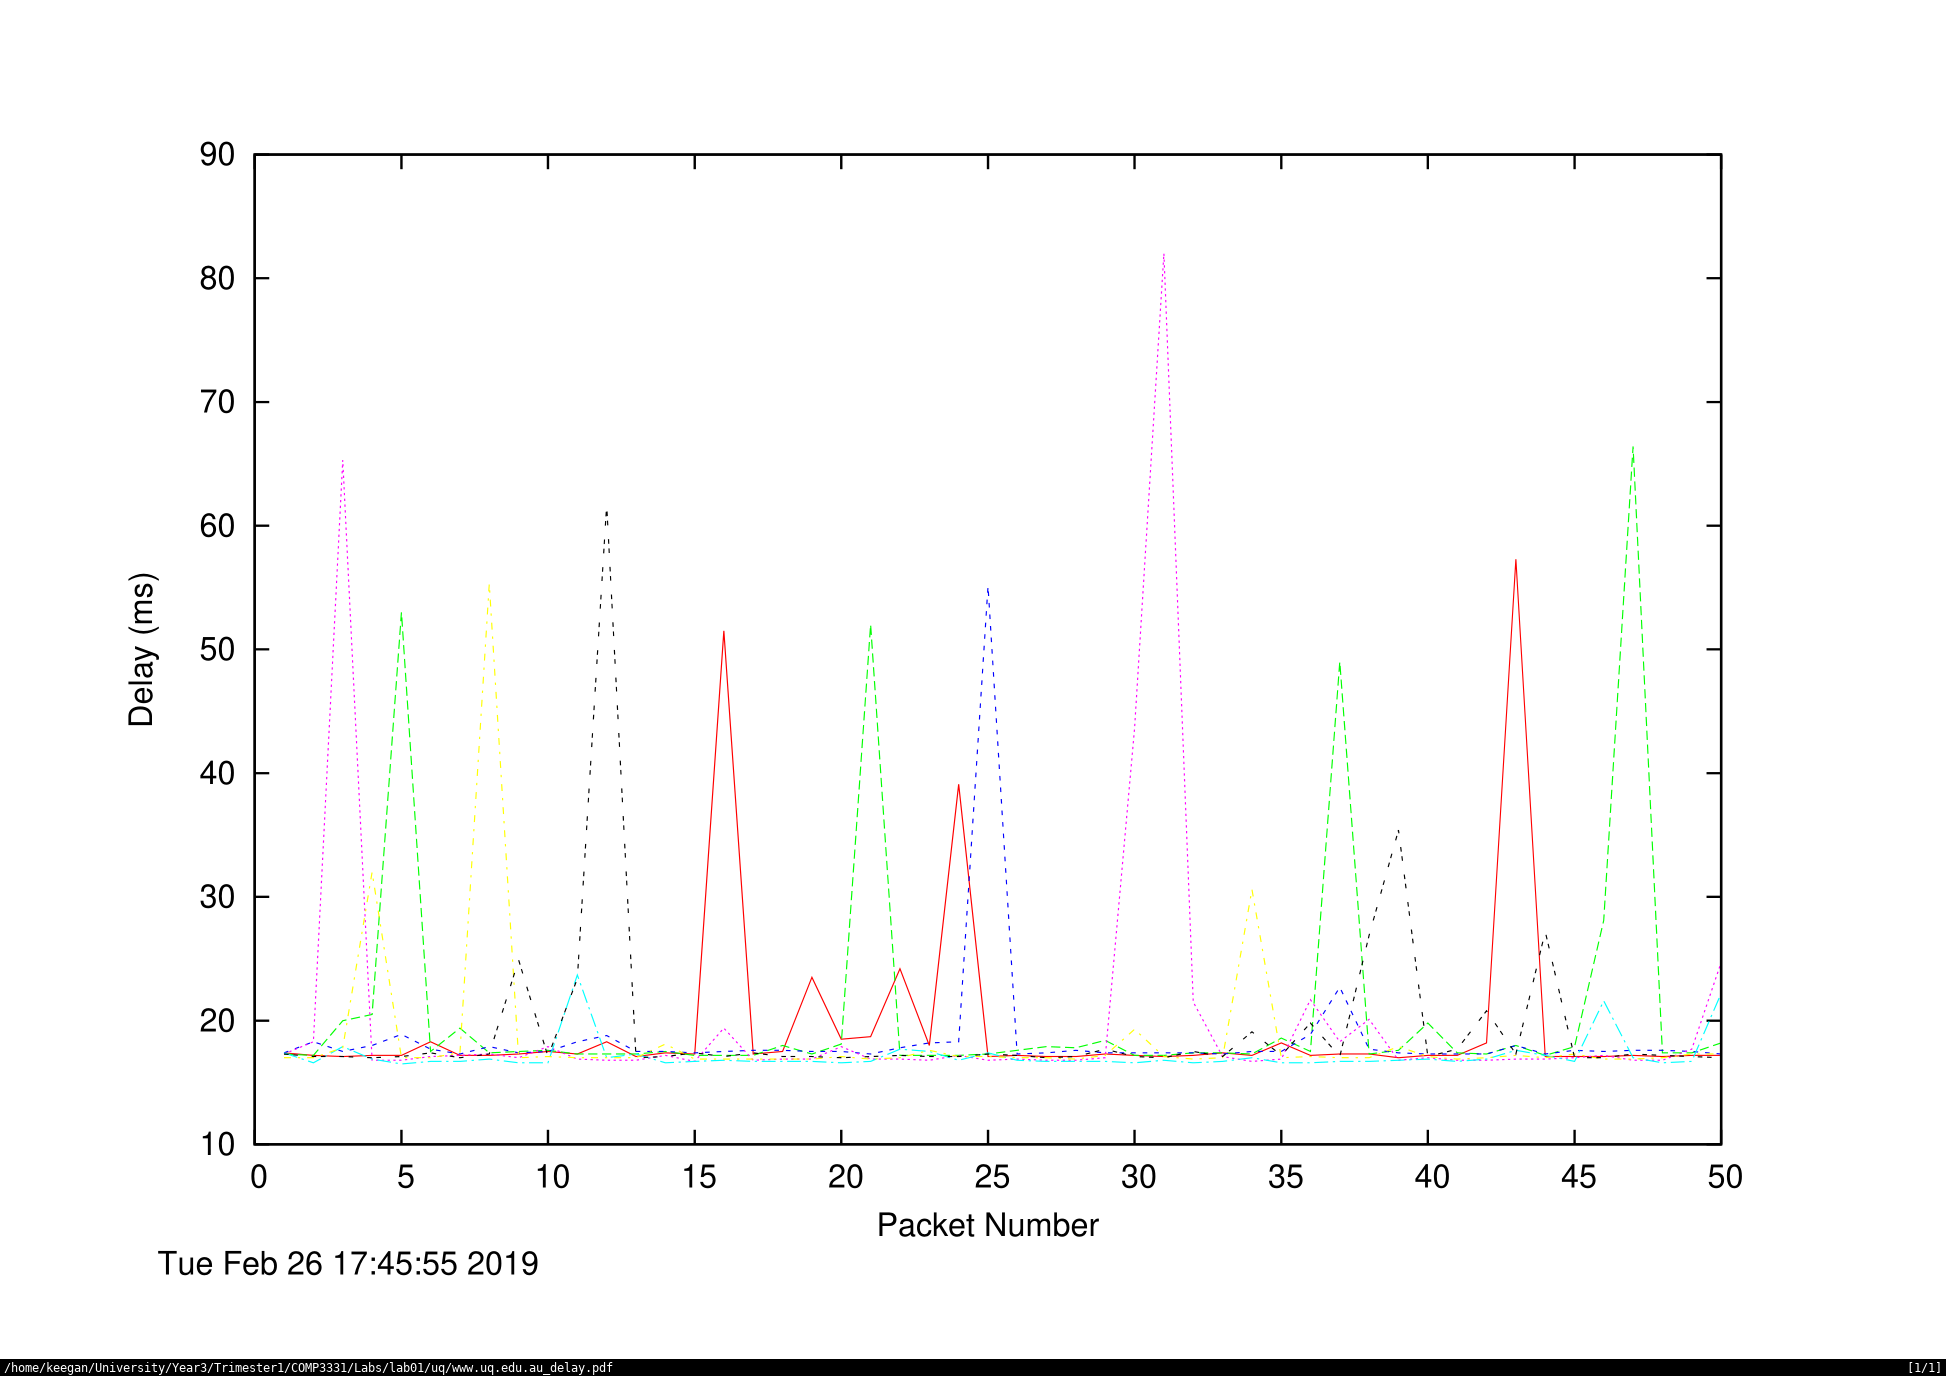
\includegraphics[width=\linewidth, height=0.43\textheight]{uqdelay.png}
		    \end{minipage}%
		\end{figure}

		\begin{figure}[!htb]
		    \centering
		    \begin{minipage}{\textwidth}
		        \centering
		        \captionof{figure}{Scatter of www.uq.edu.au vs Packet Size}
		        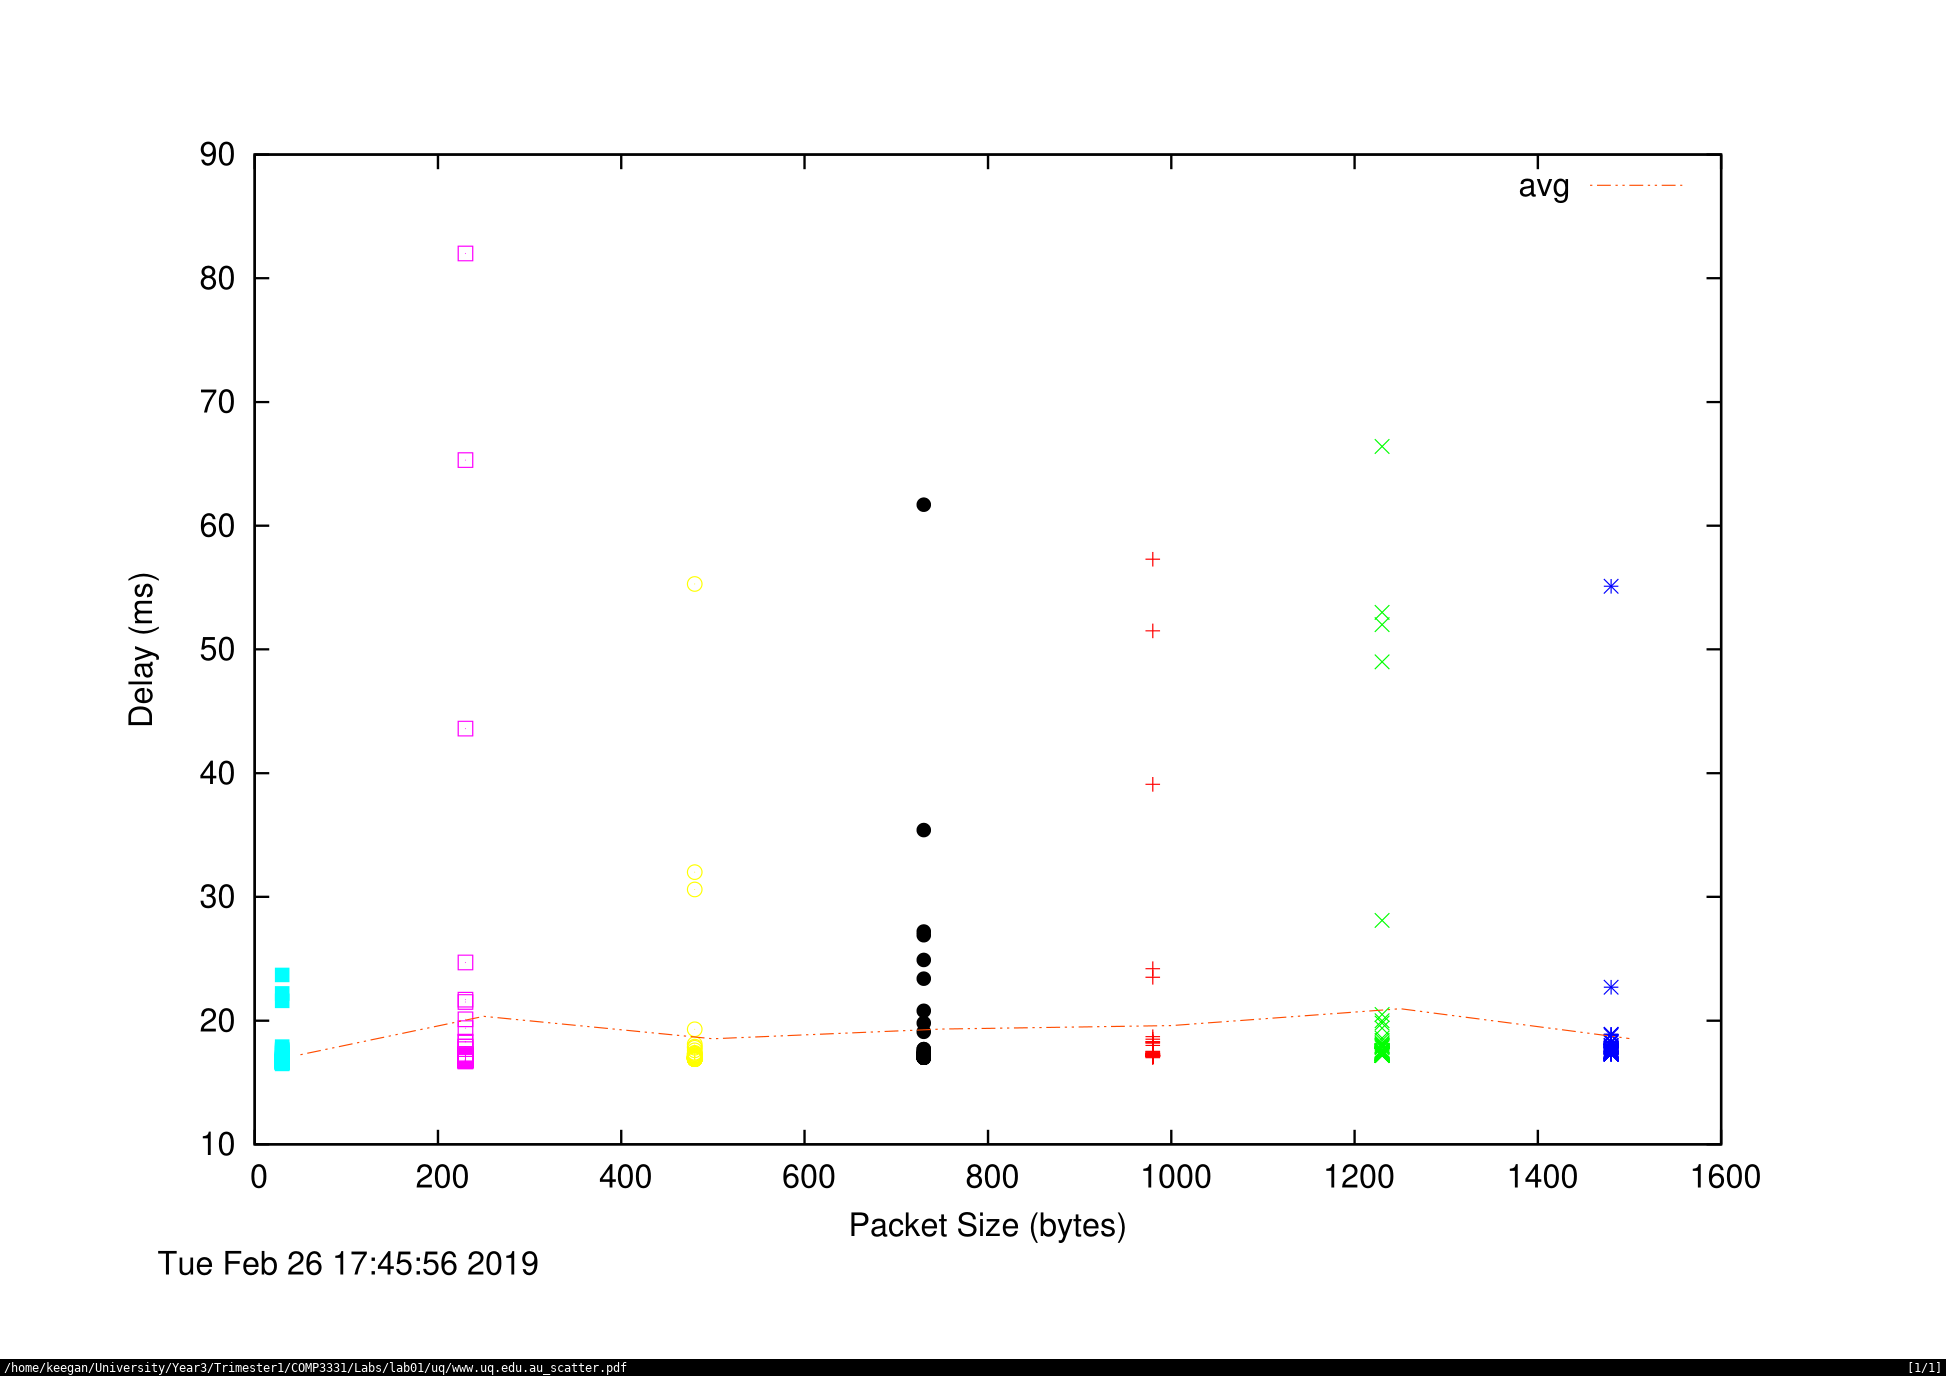
\includegraphics[width=\linewidth, height=0.43\textheight]{uqscatter.png}
		    \end{minipage}
		\end{figure}
Above are the plots from Exercise 4 provided by the \code{runping.sh} and \code{plot.sh} scripts.
\begin{enumerate}[leftmargin=*]
	\item Assume the speed of light is $\ds{3\times10^8}$m/s.
		\begin{itemize} 
			\item \textbf{University of Queenland:} Distance from UNSW is 730km. Time taken to traverse at the speed of light is 0.0024 seconds.
			\item \textbf{National University of Singapore:} Distance from UNSW is 6300km. Time taken to traverse at the speed of light is 0.021 seconds
			\item \textbf{Techniste Universitat Berlin:} Distance from UNSW is 16100km. Time taken to traverse at the speed of light is 0.054 seconds
		\end{itemize}

		\begin{figure}[!htb]
		    \centering
		    \begin{minipage}{\textwidth}
		        \centering
		        \captionof{figure}{Minimum Ping RTT / Minimum Time vs Distance}
		        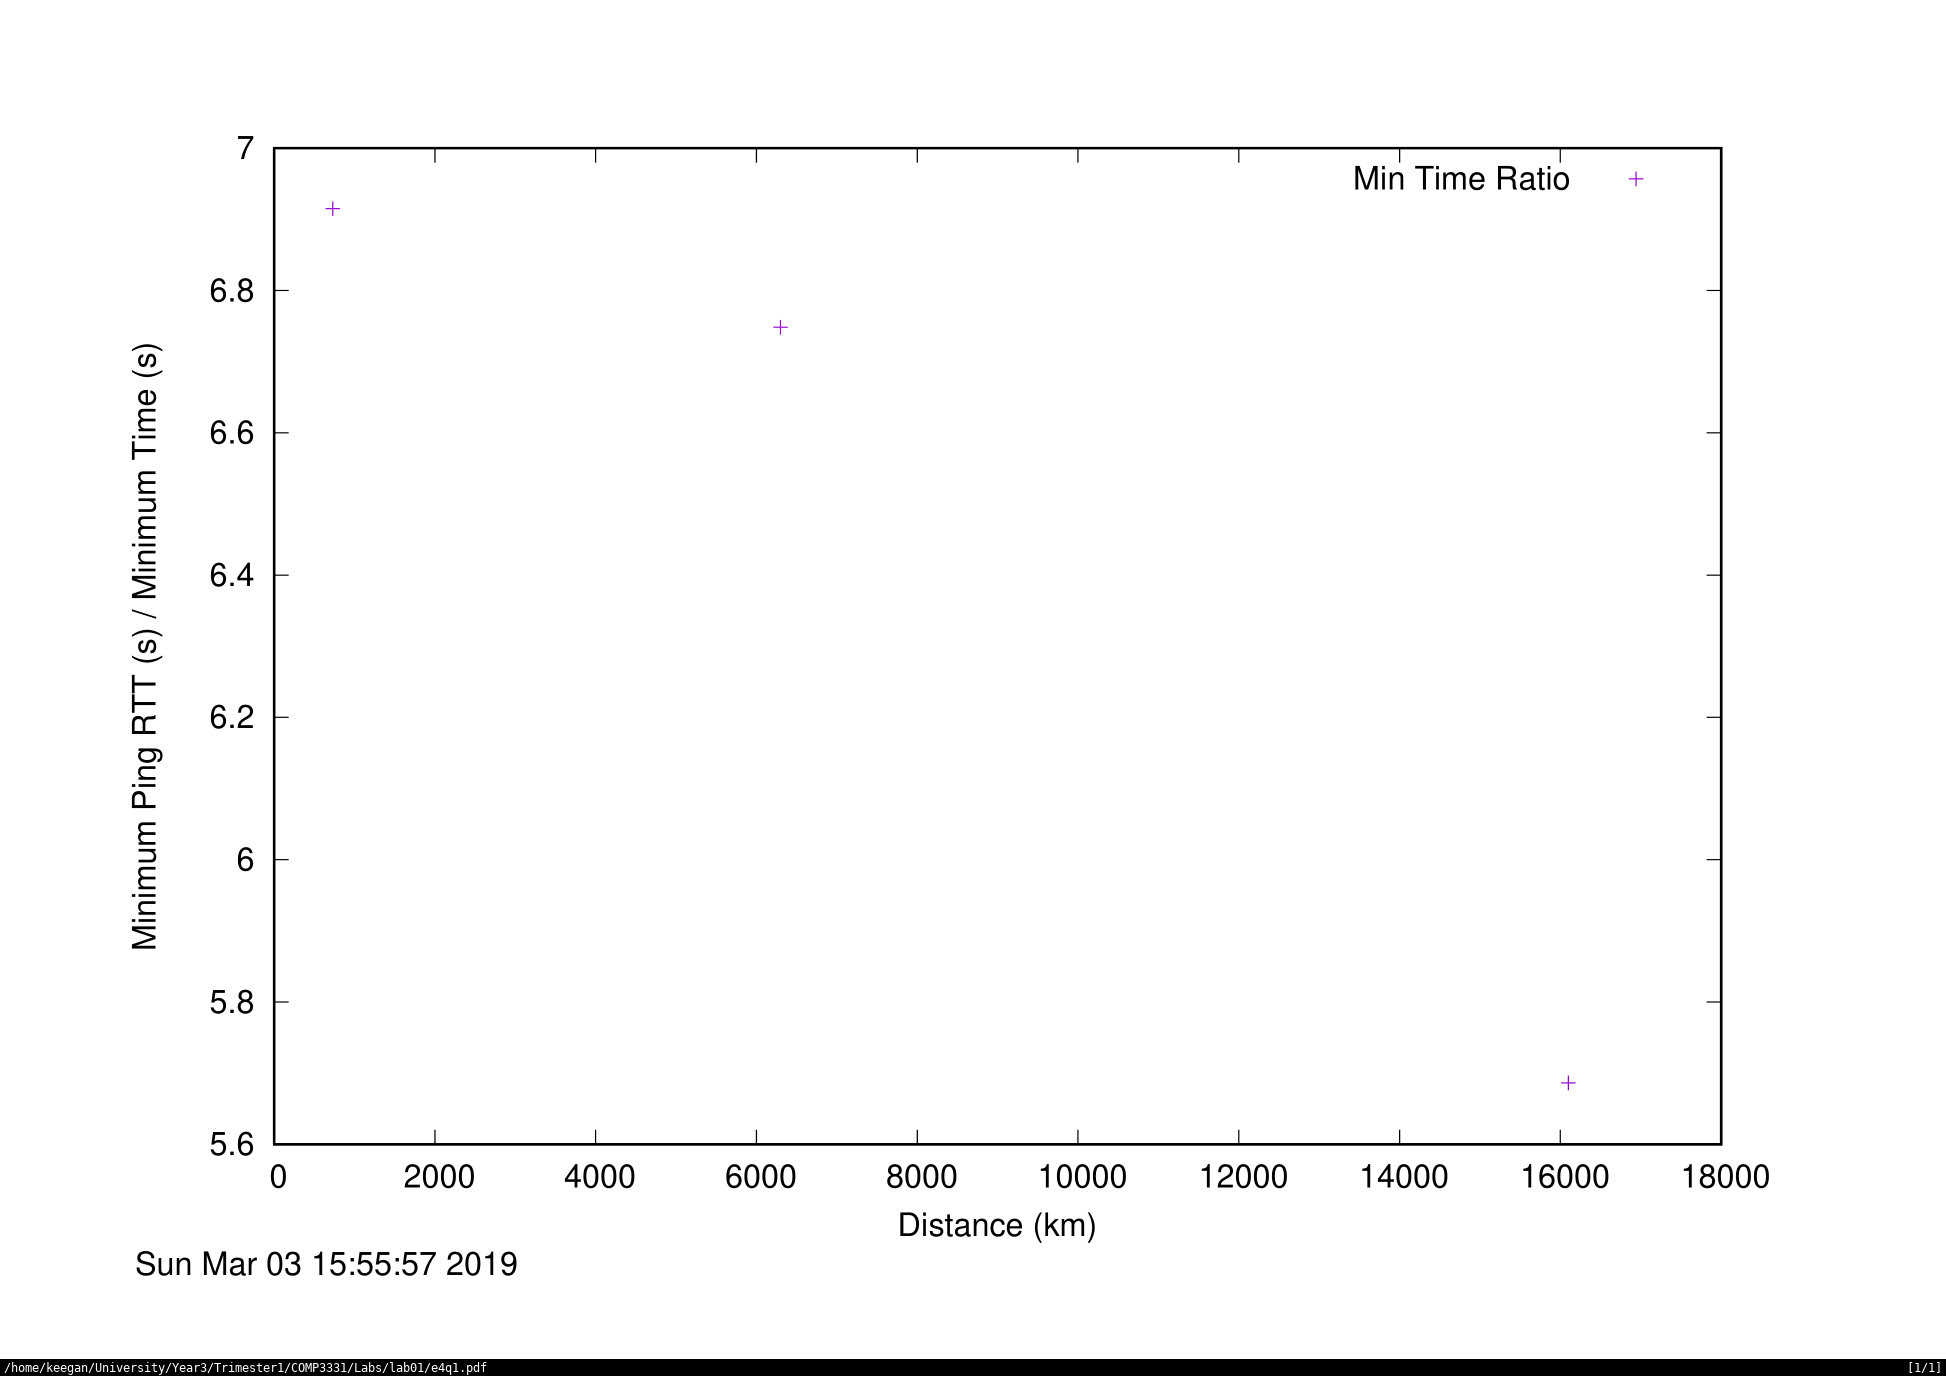
\includegraphics[width=\linewidth, height=0.5\textheight]{e4q1.png}
		    \end{minipage}
		\end{figure}

		The y-axis values are greater than $\ds{2\times T}$, where $\ds{T}$ is the time taken for the shortest distance at the speed of light, for the following reasons. Firstly, the path from the start host to the destination host is not 'as the crow flies', and so will take a longer path, and hence take longer than $\ds{2\times T}$, even if the packet was travelling at the speed of light. Secondly, the physical links are a mix of coaxial, fibre optics and other communication mediums, none of which are able to allow the packets to travel at the speed of light, and so the packet will take longer than $\ds{2\times T}$, even if the packet was travelling the most direct route.

		\pagebreak
	\item For the hosts www.uq.edu.au and www.nus.edu.sg, the delay varies signifcantly over time, especially for the host www.uq.edu.au, indicated in Figures 1 and 5 by the spikes at varying intervals across the plot. Conversely, for the www.tu-berlin.de host, the delay over time is very stable, with only 1 siginificant spike at the very end, as shown in Figure 3. However, it cannot be said that this will always be the case for the www.tu-berlin.de host. The variation in delay over time is due to the queueing delay, ie, the load on the router/host, which varies over time. This is the only delay that is affected by time, as propagation, transmission, and processing delays are all independent of time. Particular hosts may have larger spikes as other traffic may be accessing the routers/host at the same time we are pinging it. 
	\item We will consider each of the delays separately.
		\begin{itemize}
			\item \textbf{Processing Delay:} This delay is related to the packet header size and is not affected by the packet size.
			\item \textbf{Queueing Delay:} This delay is closely linked to the transmission delay, and arrival rate of packets. Packets have to wait for the time it takes to transmit those packets ahead of it, ie their transmission delay, which is dependent on packet size. However, a packet's queueing delay is not dependent on its own size, but the size of the packets in front of it in the queue, and the rate at which they all arrived.
			\item \textbf{Transmission Delay:} This delay is directly proportional to the size of the packet, as a packet's size determines how long the router takes to transmit the entire packet into the physical link.
			\item \textbf{Propagation Delay:} This delay is dependent on the distance a bit in the  packet travels, and at what speed the bit can travel, which is limited by the medium the packet is transmitted in. It is unrelated to the size of the packet.
		\end{itemize}
\end{enumerate}
\end{document}
